\pdfminorversion=6
\documentclass[12pt]{article}
\usepackage[paper=letterpaper,margin=1in]{geometry}
\usepackage{multicol}
\usepackage[utf8]{inputenc}
\usepackage{graphicx}
\usepackage{color}
\usepackage{float}
\usepackage{hyperref}

% remove lists indentation
\usepackage{enumitem}
\setlist[itemize]{leftmargin=*, itemsep=6pt, topsep=0pt, parsep=0pt}
\setlist[enumerate]{leftmargin=*, itemsep=6pt, topsep=0pt, parsep=0pt}

% discourage single lines at top/bottom of pages
\widowpenalty=10000
\clubpenalty=10000
\displaywidowpenalty=10000

%folder for graphics
\graphicspath{{./figs/}}

% pseudocode
\usepackage[linesnumbered,lined,ruled,commentsnumbered]{algorithm2e}


%%%%%%%%%%%%%%%%%%%%%%%%%%%%%%%%%%%%%%%%%%%%%%%%%%%%%%%%%%%%
\begin{document}
\begingroup
\centering
\LARGE Parallel and Distributed Computing: Homework 2\par
\vspace{10pt}
\endgroup
\noindent
\fbox{
  \parbox{\textwidth}{
    {\bf Objectives} : Use an isolated computer network to expose the layered OSI model of communications. The student is challenged to connect two virtual computers in a single machine, to follow the packets of two communicating processes and identify the OSI layers used in the communications mechanism. Using the C programming language, and a network `sniffer," two processes will be defined and communicate in a ``client-server" configuration to identify the layers packets traverse during the communications. Bit patterns will be identified to answer questions related to the exercise.}
}
\vspace*{15pt}

\begin{em}
  ``A protocol stack (such as OSI), today is usually provided by the operating system (rather than as a separate library, for instance), it is a set of programs that allow processes to communicate over a network using the protocols that the stack implements.
  
  The application programming interface (API) that programs use to communicate with the protocol stack, using network sockets, is called a socket API. Development of application programs that utilize this API is called socket programming or network programming.''
\end{em}
\rightline{\url{https://en.wikipedia.org/wiki/Network_socket}}

\vspace{15pt}

%============================================================================
\begin{multicols}{2}
\subsection*{Assignment}
Install Virtualbox in your computer.
Create two new Virtual Machines (VMs) \textbf{TX} and \textbf{RX}; they will act as TCP client and TCP server respectively.
Use some lightweight Linux distribution such as Xubuntu in each of them. Little RAM and one core per VM should be enough.
Configure their shared virtual network so that both VMs share the same network segment. This is a \href{https://youtu.be/vReAkOq-59I}{good tutorial} on YouTube.
Install \href{https://www.wireshark.org/docs/}{Wireshark} in \textbf{RX}. {\color{red}Note that the use of Wireshark in any UCI network is forbidden. \textbf{Do not} use Wireshark or any other sniffing tool in any UCI network.}

Create a C program \texttt{tx.c} in \textbf{TX}.
Create a C program \texttt{rx.c} in \textbf{RX}.
The first part of your assignment is, using \textbf{sockets}, make the TCP client \textbf{TX} send a (perhaps even hard-coded) short message such as ``\texttt{Hello Sockets}'' to the TCP server \textbf{RX}.


\paragraph{Capturing packets:}
On \textbf{RX}, run the \texttt{rx} program. Then, start capturing packages with Wireshark.
In \textbf{TX}, run the \texttt{tx} program to send the message.
There are plenty of guides and tutorials on the web on how to use sockets to send messages across two machines in Linux.

When you start capturing packets, make sure of selecting the appropiate interface. Services, browser, and the OS constantly send packets to the Internet and the local network, therefore, in order to capture only the packet of interest, you will need to apply a \textbf{capture filter, NOT A DISPLAY FILTER}. Something like this:

\centerline{``\texttt{ip src TX\_IP and ip dst RX\_IP}''}
  
Where \texttt{TX\_IP} and \texttt{RX\_IP} are the IP addresses of \textbf{TX} and \textbf{RX} VMs.

\subsection*{Report}
Write a report of 2 pages. {\em Do not forget to include your name and student ID number on the top of the first page of your report.}

\paragraph{First page:} identify the single packet that contains the message sent from \textbf{TX} to \textbf{RX}. Based on this packet, \textbf{concisely} answer the following questions. Note that ``A-B'' denotes the inclusive range from A to B:

\begin{itemize}
\item What is encoded, and what is the purpose of bytes 0-5 and 6-11?
\item What is encoded, and what is the relationship between, byte 14 and the two bytes 16,17?
\item What is encoded, and what is the purpose of bytes 18-19?
\item What is encoded, and what is the purpose of bytes 20-21?
\item What is encoded, and what is the purpose of byte 23?
\item What is encoded, and what is the purpose of bytes 26-29 and 30-33?
\item What is encoded, and what is the purpose of bytes 34-35 and 36-37?
\item What is encoded  after byte 65?
\end{itemize}

%===========================================================
\begin{figure}[H]
  %%\vspace{45pt}
  \centering
  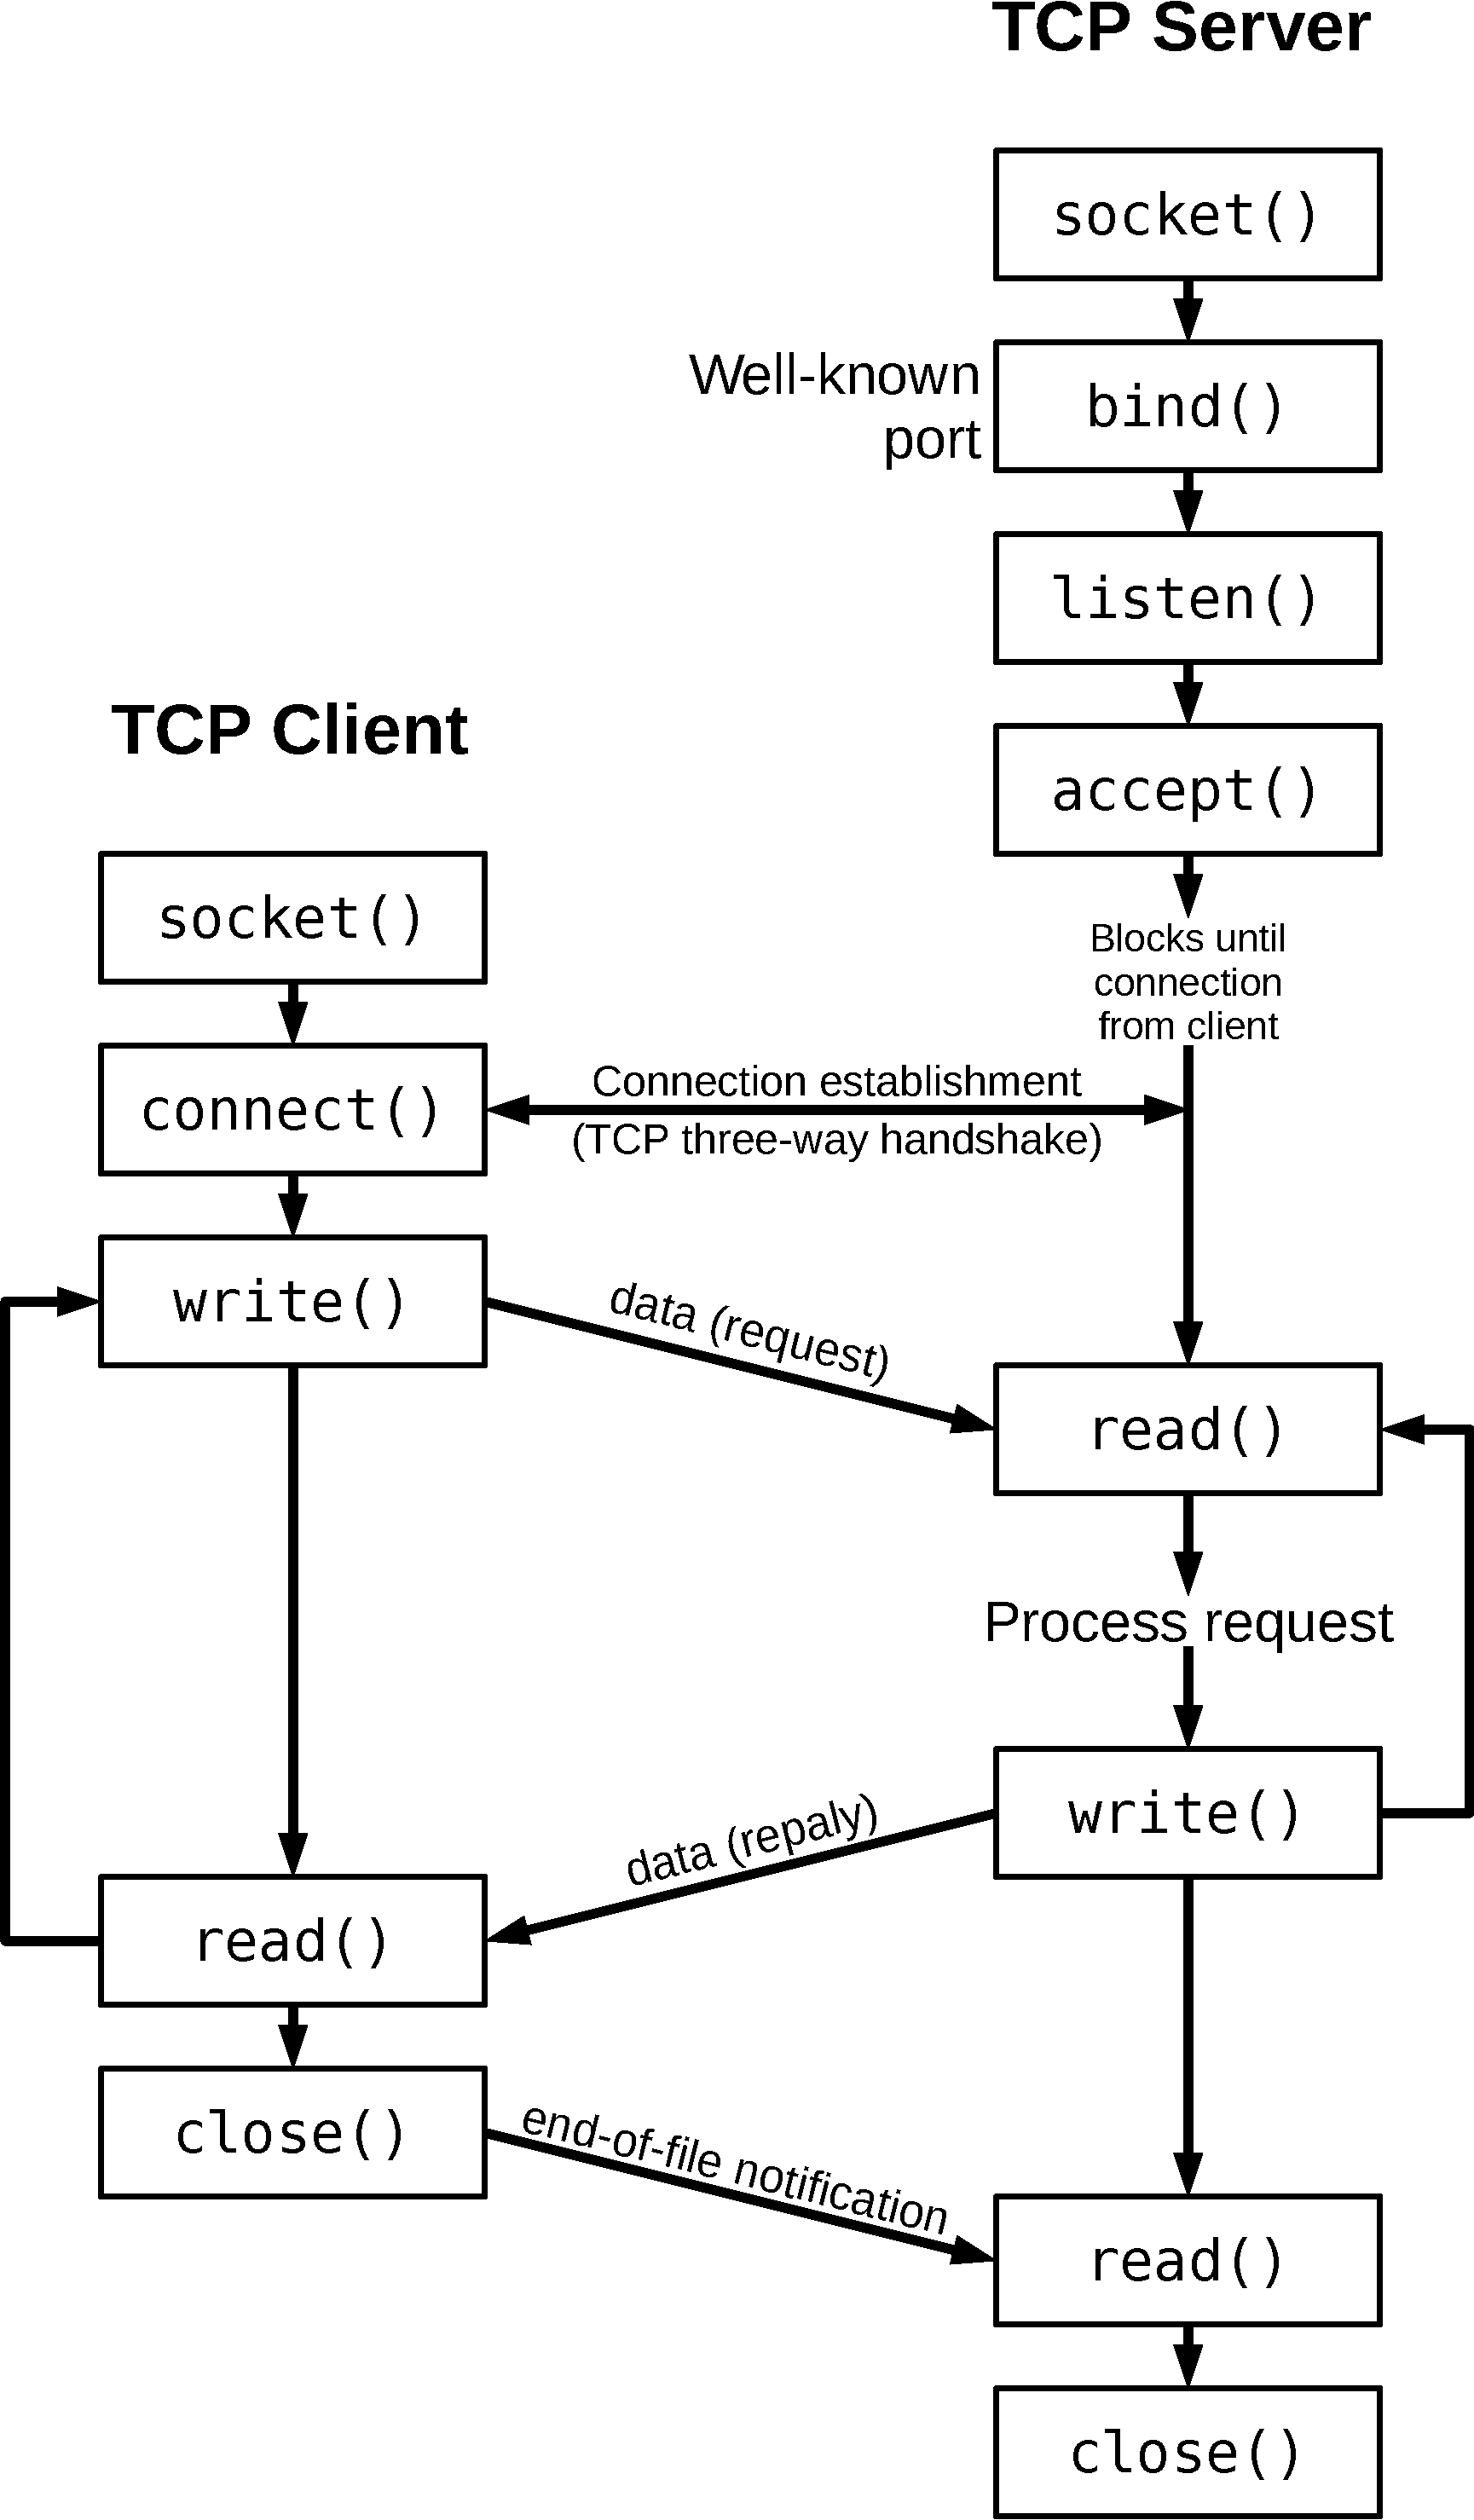
\includegraphics[width=0.75\linewidth]{tcp_client_server}
  \caption*{\scriptsize After ``Unix Network Programming''\\by W. Richard Stevens}
\end{figure}
%===========================================================


Please note that we are asking you to identify \textbf{what is} and to briefly explain \textbf{the PURPOSE} of each group of bytes.

\paragraph{Second page:} Obtain a clear screenshot of the raw block of bits of the previously mentioned single packet that contains the message sent by \texttt{Client} (raw blocks are located at the bottom part of Wireshark's window).

Split that block of bits, include it on the report, and associate each partition of bits to the layers 2 (Link), 3 (Network), 4 (Transport), and 7 (Application); by indicating the first and last byte of each layer, as an inclusive range ``A-B''.

%===========================================================
\subsection*{Submission}
Submit \textbf{one} zip file named \texttt{hw2.zip}, containing \textbf{exactly 5 files}. Make sure the zip file does \textbf{not} include sub-directories (as Mac's default compression tool does) or extra files:

\begin{enumerate}
\item \texttt{tx.c}: The commented C source code of the client VM.
\item \texttt{rx.c}: The commented C source code of the server VM.
\item \texttt{packets.pcapng}: The captured packets in \texttt{pcapng} format. The file \textbf{must only} contain packets transmitted between \textbf{TX} and \textbf{RX} VMs. This file \textbf{cannot weight more than a few kilobytes}. If that is the case, then you did not filter the capture and will obtain 0 points in this section.
\item  \texttt{report.pdf}: The digitally produced report.
\item \texttt{team.txt}: Text file with two lines containing the UCINetID and name of each student in your team:\\
  \texttt{<UCINetID> <firstName> <lastName>}
\end{enumerate}

\end{multicols}
\end{document}
